\documentclass[11pt]{article}
\usepackage[margin=0.7in]{geometry} 
\usepackage{amsmath,amsthm,amssymb,amsfonts, amsbsy}
\usepackage{enumitem}
\usepackage{dsfont}
\usepackage{soul}
\usepackage{mathtools}
\usepackage[utf8]{inputenc}
\usepackage{multirow}
\usepackage[colorlinks]{hyperref}
\usepackage{cleveref}
\usepackage{bbm}
\usepackage{tikz-cd}
\usepackage{adjustbox}
\usepackage[normalem]{ulem}
\usepackage{authblk}
\usepackage{listings}
\usepackage{xcolor}
\usepackage{graphicx}

\renewcommand{\baselinestretch}{1.25}

\definecolor{codegreen}{rgb}{0,0.6,0}
\definecolor{codegray}{rgb}{0.5,0.5,0.5}
\definecolor{codepurple}{rgb}{0.58,0,0.82}
\definecolor{backcolour}{rgb}{0.95,0.95,0.92}

\lstdefinestyle{mystyle}{
    backgroundcolor=\color{backcolour},   
    commentstyle=\color{codegreen},
    keywordstyle=\color{magenta},
    numberstyle=\tiny\color{codegray},
    stringstyle=\color{codepurple},
    basicstyle=\ttfamily\footnotesize,
    breakatwhitespace=false,         
    breaklines=true,                 
    captionpos=b,                    
    keepspaces=true,                 
    numbers=left,                    
    numbersep=5pt,                  
    showspaces=false,                
    showstringspaces=false,
    showtabs=false,                  
    tabsize=2
}

\lstset{style=mystyle}
 
\newtheorem{lemma}{Lemma}
\newtheorem{claim}{\sf Claim}
\newtheorem{defi}{Definition}
\newtheorem{thm}{Theorem}
\newtheorem{cor}{Corollary}
\newtheorem{prop}{Proposition}
\newtheorem{rmk}{\it Remark}
\newtheorem{ex}{Example}
\newtheorem{notation}{Notation}
\newtheorem{algorithm}{Algorithm}
\newtheorem{assumption}{Assumption}
\newtheorem{problem}{Problem}

\DeclareMathOperator*{\argmin}{argmin}
\DeclareMathOperator*{\argmax}{argmax}

\numberwithin{equation}{problem}
  
\begin{document}
 
\title{MAS374 Optimization theory\\ Homework \#4}
\author{20150597 Jeonghwan Lee}
\affil{Department of Mathematical Sciences, KAIST}

\maketitle

\begin{problem} [\emph{Exercise 6.1} in \cite{calafiore2014optimization}: Least-squares and total least-squares]
\label{problem1}
\normalfont{\ \\
\indent Let
\begin{equation*}
    \mathbf{X} := 
    \begin{bmatrix}
        1 & x_1 \\ 1 & x_2 \\ 1 & x_3 \\ 1 & x_4
    \end{bmatrix}
    =
    \begin{bmatrix}
        1 & -1 \\ 1 & 0 \\ 1 & 1 \\ 1 & 2
    \end{bmatrix}
    \in \mathbb{R}^{4 \times 2} \quad \textnormal{and} \quad
    \mathbf{y} :=
    \begin{bmatrix}
        y_1 \\ y_2 \\ y_3 \\ y_4
    \end{bmatrix}
    =
    \begin{bmatrix}
        0 \\ 0 \\ 1 \\ 1
    \end{bmatrix}
    \in \mathbb{R}^4.
\end{equation*}
We first find the least-squares (\textsf{LS}) line for the given data-set $\left\{ \left( x_i, y_i \right) \in \mathbb{R}^2 : i \in [4] \right\}$. The \textsf{LS} problem seeks for the line $y = \theta_{0}^{\textsf{LS}} + \theta_{1}^{\textsf{LS}} x$ that matches with the given data-set most well by minimizing the \emph{sum of squared residuals}:
\begin{equation}
    \label{eqn1.1}
    \min_{\left( \theta_0, \theta_1 \right) \in \mathbb{R}^2} \ 
    \sum_{i=1}^{4} \left\{ y_i - \left( \theta_0 + \theta_1 x \right) \right\}^2 = \left\| \mathbf{y} - \mathbf{X} \boldsymbol{\theta} \right\|_{2}^2,
\end{equation}
where $\boldsymbol{\theta} = \begin{bmatrix} \theta_0 \\ \theta_1 \end{bmatrix} \in \mathbb{R}^2$. So it suffices to find the optimal solution $\boldsymbol{\theta}^{\textsf{LS}} = \begin{bmatrix} \theta_{0}^{\textsf{LS}} \\ \theta_{1}^{\textsf{LS}} \end{bmatrix} \in \mathbb{R}^2$ to the \textsf{LS} problem \eqref{eqn1.1}. It's clear that $\mathbf{X} \in \mathbb{R}^{4 \times 2}$ has full column-rank, thereby $\mathbf{X}^{\top} \mathbf{X} \in \mathbb{R}^{2 \times 2}$ is invertible. From the normal equation $\mathbf{X}^{\top} \left( \mathbf{y} - \mathbf{X} \boldsymbol{\theta}^{\textsf{LS}} \right) = \mathbf{0}$, one has
\begin{equation}
    \label{eqn1.2}
    \boldsymbol{\theta}^{\textsf{LS}} = \left( \mathbf{X}^{\top} \mathbf{X} \right)^{-1} \mathbf{X}^{\top} \mathbf{y} =
    \begin{bmatrix}
        \frac{3}{10} \\ \frac{2}{5}
    \end{bmatrix}
    \in \mathbb{R}^2.
\end{equation}
Thus, the least-squares (\textsf{LS}) line for the given data-set is given by
\begin{equation}
    \label{eqn1.3}
    y = \theta_{0}^{\textsf{LS}} + \theta_{1}^{\textsf{LS}} x = \frac{3}{10} + \frac{2}{5} x = 0.3 + 0.4 x.
\end{equation}
\medskip
\indent We next look for the total least-squares (\textsf{TLS}) line for the given data-set $\left\{ \left( x_i, y_i \right) \in \mathbb{R}^2 : i \in [4] \right\}$. To this end, we first consider the linear system $\mathbf{y} = \mathbf{X} \boldsymbol{\theta}$. We note that the \textsf{LS} problem can be interpreted as follows: find a \emph{minimal perturbation} $\delta \mathbf{y} \in \mathbb{R}^4$ in the $\mathbf{y}$ term so that the linear system $\mathbf{y} + \delta \mathbf{y} = \mathbf{X} \boldsymbol{\theta}$ becomes feasible, \emph{i.e.},
\begin{equation}
    \label{eqn1.4}
    \begin{split}
        \min_{\delta \mathbf{y} \in \mathbb{R}^4} \ &\left\| \delta \mathbf{y} \right\|_{2}^2 \\
        \textnormal{subject to }\ &\mathbf{y} + \delta \mathbf{y} \in \mathcal{R} \left( \mathbf{X} \right).
    \end{split}
\end{equation}
This interpretation of the \textsf{LS} problem was covered in our lectures.
\medskip

\indent On the other hand, the total least-squares (\textsf{TLS}) approach extends this interpretation of the \textsf{LS} problem by allowing the perturbation to act both on the $\mathbf{y}$ term and on the $\mathbf{X}$ matrix. The \textsf{TLS} problem searches for the pair of \emph{minimal perturbations} $\delta \mathbf{X} \in \mathbb{R}^{4 \times 2}$ and $\delta \mathbf{y} \in \mathbb{R}^4$ in the $\mathbf{X}$ matrix and the $\mathbf{y}$ term, respectively, so that the linear system $\mathbf{y} + \delta \mathbf{y} = \left( \mathbf{X} + \delta \mathbf{X} \right) \boldsymbol{\theta}$ is feasible, \emph{i.e.}, 
\begin{equation}
    \label{eqn1.5}
    \begin{split}
        \min_{\left( \delta \mathbf{X}, \delta \mathbf{y} \right) \in \mathbb{R}^{4 \times 2} \times \mathbb{R}^4} \ &\left\|
        \begin{bmatrix}
            \delta \mathbf{X} & \delta \mathbf{y}
        \end{bmatrix}
        \right\|_{\textsf{F}}^2 \\
        \textnormal{subject to }\ &\mathbf{y} + \delta \mathbf{y} \in \mathcal{R} \left( \mathbf{X} + \delta \mathbf{X} \right).
    \end{split}
\end{equation}
Let $\mathbf{A} := \begin{bmatrix} \mathbf{X} & \mathbf{y} \end{bmatrix} \in \mathbb{R}^{4 \times 3}$ and $\delta \mathbf{A} := \begin{bmatrix} \delta \mathbf{X} & \delta \mathbf{y} \end{bmatrix}$. For the given data-set, we have
\begin{equation*}
    \mathbf{A} =
    \begin{bmatrix}
        1 & -1 & 0 \\ 1 & 0 & 0 \\ 1 & 1 & 1 \\ 1 & 2 & 1
    \end{bmatrix}.
\end{equation*}
Then, $\mathbf{A}$ satisfies the technical assumptions required for the validity of \emph{Theorem 6.2} in \cite{calafiore2014optimization}:
\begin{enumerate} [label=(\roman*)]
    \item $\textsf{rank} (\mathbf{A}) = 3$;
    \item $\sigma_{3} (\mathbf{A}) = \sigma_{\min} (\mathbf{A}) < \sigma_{\min} (\mathbf{X})$.
\end{enumerate}
It is straightforward to see that the assumption (\romannumeral 1) holds. So it remains to verify that the assumption (\romannumeral 2) holds. From
\begin{equation*}
    \mathbf{A}^{\top} \mathbf{A} =
    \begin{bmatrix}
        4 & 2 & 2 \\ 2 & 6 & 3 \\ 2 & 3 & 2
    \end{bmatrix} \quad \textnormal{and} \quad
    \mathbf{X}^{\top} \mathbf{X} =
    \begin{bmatrix}
        4 & 2 \\ 2 & 6
    \end{bmatrix}
\end{equation*}
together with the observations $\sigma_i (\mathbf{A}) = \sqrt{\lambda_i \left( \mathbf{A}^{\top} \mathbf{A} \right)}$ for $i \in [3]$, and $\sigma_j (\mathbf{X}) = \sqrt{\lambda_i \left( \mathbf{X}^{\top} \mathbf{X} \right)}$ for $j \in [2]$, one can compute both $\sigma_{\min} (\mathbf{A})$ and $\sigma_{\min} (\mathbf{X})$ numerically:
\begin{equation*}
    \begin{split}
        \sigma_{\min} (\mathbf{A})^2 &= \sigma_{3} (\mathbf{A})^2 = \lambda_3 \left( \mathbf{A}^{\top} \mathbf{A} \right) \approx 0.15927314; \\
        \sigma_{\min} (\mathbf{X})^2 &= \sigma_{2} (\mathbf{X})^2 = \lambda_2 \left( \mathbf{X}^{\top} \mathbf{X} \right) = 4 - \sqrt{13} \approx 0.39444872,
    \end{split}
\end{equation*}
thereby the assumption (\romannumeral 2) holds. At this moment, we note that the eigenvalues of the $3 \times 3$ positive definite matrix $\mathbf{A}^{\top} \mathbf{A}$ (as well as the singular values of $\mathbf{A}$) should be computed numerically, since the characteristic polynomial $\textsf{ch}_{\mathbf{A}^{\top} \mathbf{A}}(x) := \textsf{det} \left( x \mathbf{I}_3 - \mathbf{A}^{\top} \mathbf{A} \right)$ of $\mathbf{A}^{\top} \mathbf{A}$ is irreducible over the rational number field $\mathbb{Q}$:
\begin{equation*}
    \textsf{ch}_{\mathbf{A}^{\top} \mathbf{A}}(x) = x^3 - 12 x^2 + 27 x - 4.
\end{equation*}
To this end, for instance, I made use of the function \href{https://numpy.org/doc/stable/reference/generated/numpy.linalg.svd.html}{\texttt{np.linalg.svd}} in Python 3. 
\medskip

\indent From \emph{Theorem 6.2} in \cite{calafiore2014optimization}, we find that the \textsf{TLS} problem \eqref{eqn1.5} has the unique optimal solution $\left( \left( \delta \mathbf{X} \right)^*, \left( \delta \mathbf{y} \right)^* \right) \in \mathbb{R}^{4 \times 2} \times \mathbb{R}^4$ and it satisfies
\begin{equation*}
    \left( \delta \mathbf{A} \right)^* =
    \begin{bmatrix}
        \left( \delta \mathbf{X} \right)^* & \left( \delta \mathbf{y} \right)^*
    \end{bmatrix}
    = - \sigma_3 ( \mathbf{A} ) \cdot \mathbf{u}_3 \mathbf{v}_{3}^{\top},
\end{equation*}
where $\mathbf{A} = \sum_{i=1}^{3} \sigma_i (\mathbf{A}) \cdot \mathbf{u}_i \mathbf{v}_{i}^{\top}$ is the compact-form \textsf{SVD} of $\mathbf{A} \in \mathbb{R}^{4 \times 3}$. Moreover, the solution $\boldsymbol{\theta}^{\textsf{TLS}} \in \mathbb{R}^2$ of the feasible linear system $\mathbf{y} + \left( \delta \mathbf{y} \right)^* = \left\{ \mathbf{X} + \left( \delta \mathbf{X} \right)^* \right\} \boldsymbol{\theta}$ uniquely exists, and it is given by
\begin{equation}
    \label{eqn1.6}
    \begin{split}
        \boldsymbol{\theta}^{\textsf{TLS}} &= \left\{ \mathbf{X}^{\top} \mathbf{X} - \sigma_{\min} (\mathbf{A})^2 \mathbf{I}_2 \right\}^{-1} \mathbf{X}^{\top} \mathbf{y} \\
        &= \frac{1}{20 - 10 \sigma_{\min} (\mathbf{A})^2 + \sigma_{\min} (\mathbf{A})^4}
        \begin{bmatrix}
            6 - 2\sigma_{\min} (\mathbf{A})^2 \\ 8 - 3\sigma_{\min} (\mathbf{A})^2
        \end{bmatrix} \\
        &\approx
        \begin{bmatrix}
            0.30822795 \\ 0.40809032
        \end{bmatrix},
    \end{split}
\end{equation}
where the approximated value in \eqref{eqn1.6} is computed numerically via the functions \href{https://numpy.org/doc/stable/reference/generated/numpy.linalg.inv.html}{\texttt{np.linalg.inv}} and \href{https://numpy.org/doc/stable/reference/generated/numpy.linalg.svd.html}{\texttt{np.linalg.svd}} in Python 3. Therefore, the total-least squares (\textsf{TLS}) line for the given data-set is
\begin{equation}
    \label{eqn1.7}
    y = \theta_{0}^{\textsf{TLS}} + \theta_{1}^{\textsf{TLS}} x
    \approx 0.30822795 + 0.40809032x.
\end{equation}
\medskip

\indent Finally, we plot both the \textsf{LS} line \eqref{eqn1.3} and the \textsf{TLS} line \eqref{eqn1.7} on the same set of axes. It can be done by using the following code in Python 3:
\begin{lstlisting}[language = Python]
import numpy as np
import matplotlib as mpl
import matplotlib.pyplot as plt

def axes():
    plt.axhline(0, alpha=.1)
    plt.axvline(0, alpha=.1)
    
dataset_x = np.array([-1, 0, 1, 2])
dataset_y = np.array([0, 0, 1, 1])
X = np.transpose(np.stack([np.ones(len(dataset_x)), dataset_x]))
theta_LS = np.linalg.lstsq(X, dataset_y, rcond=None)[0]
print(theta_LS)

M = np.transpose(np.stack([np.ones(len(dataset_x)), dataset_x, dataset_y]))
u, s, vh = np.linalg.svd(M, full_matrices=False)
min_singular_M = s[2]
theta_TLS = np.dot(np.linalg.inv(np.dot(np.transpose(X), X) - (min_singular_M**2)*np.identity(2)), np.dot(np.transpose(X), dataset_y))
print(theta_TLS)

axes()
_ = plt.plot(dataset_x[0], dataset_y[0], 'o', label='Data point 1', markersize=4)
_ = plt.plot(dataset_x[1], dataset_y[1], 'o', label='Data point 2', markersize=4)
_ = plt.plot(dataset_x[2], dataset_y[2], 'o', label='Data point 3', markersize=4)
_ = plt.plot(dataset_x[3], dataset_y[3], 'o', label='Data point 4', markersize=4)
_ = plt.plot(dataset_x, theta_LS[0] + theta_LS[1]*dataset_x, label='Least-squares line')
_ = plt.plot(dataset_x, theta_TLS[0] + theta_TLS[1]*dataset_x, label='Total least-squares line')
_ = plt.legend()
plt.show()
\end{lstlisting}
This code results in the following visualization:
\begin{figure}[h]
    \centering
    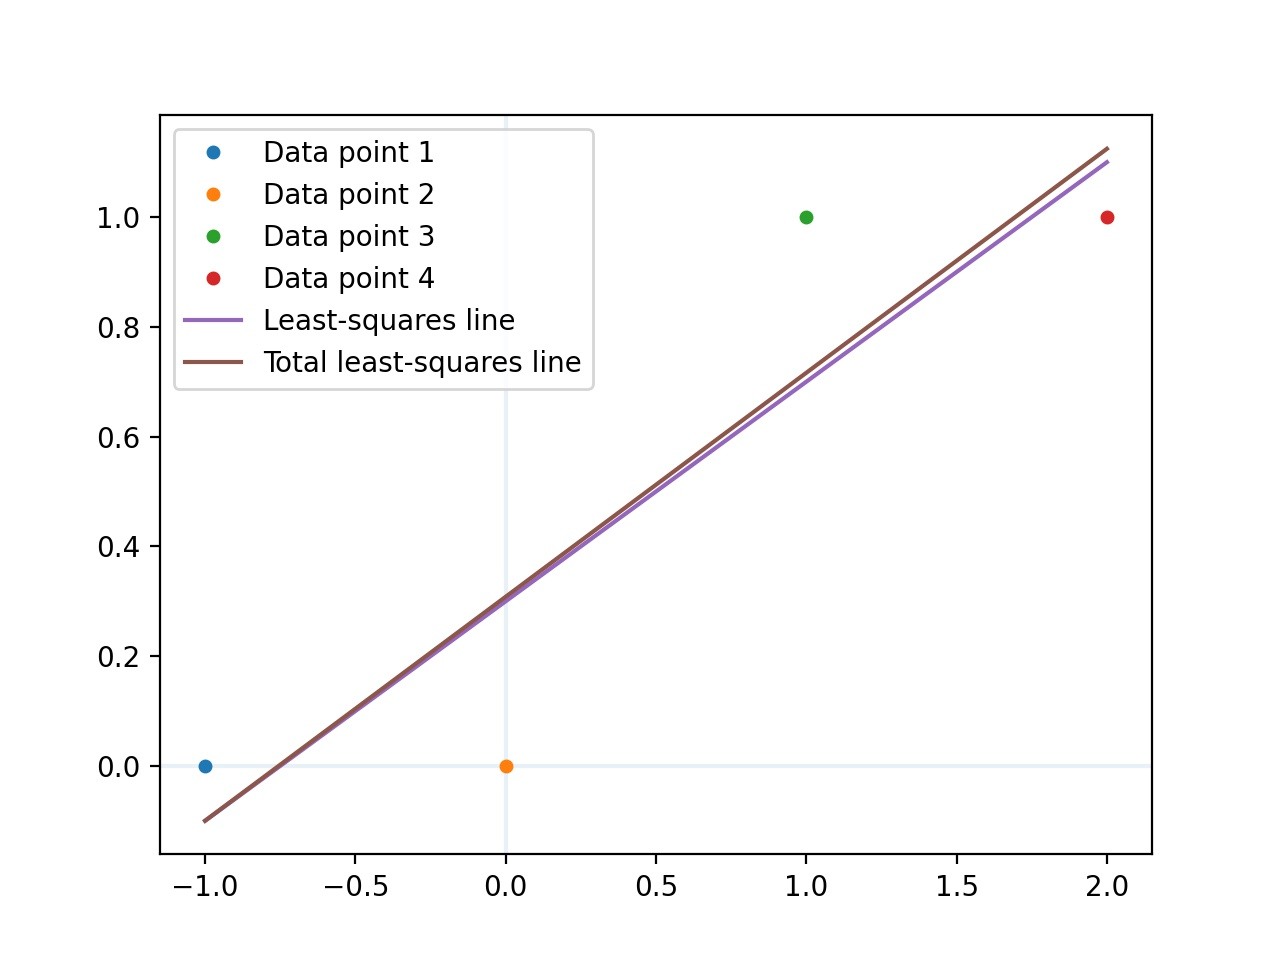
\includegraphics[width=0.6\textwidth]{HW4/figure_problem1.jpg}
    \caption{Visualization of both the least-squares line and the total least-squares line in Problem \ref{problem1}}
    \label{fig:problem_1}
\end{figure}
}
\end{problem}

\begin{problem} [\emph{Exercise 6.2} in \cite{calafiore2014optimization}: Geometry of least-squares problems]
\label{problem2}
\normalfont{\ \\
\indent To begin with, let $\mathcal{X}_{\textsf{opt}} := \argmin \left\{ \left\| \mathbf{y} - \mathbf{A} \mathbf{x} \right\|_2 : \mathbf{x} \in \mathbb{R}^n \right\}$. Due to the projection theorem (\emph{Theorem 2.2} in \cite{calafiore2014optimization}), we have $\mathcal{X}_{\textsf{opt}} \neq \varnothing$ and if $\mathbf{x}^* \in \mathcal{X}_{\textsf{opt}}$, then
\begin{equation}
    \label{eqn2.1}
    \mathbf{y} - \mathbf{A} \mathbf{x}^* \perp \mathcal{R} (\mathbf{A}).
\end{equation}
In order to discuss the properties of the residual vector $\mathbf{r} := \mathbf{y} - \mathbf{A} \mathbf{x}^* \in \mathbb{R}^m$ at an optimal solution, we first establish the well-definedness of the residual vector. In other words, we claim that
\begin{equation}
    \label{eqn2.2}
    \mathbf{y} - \mathbf{A} \mathbf{x}_{1}^* = \mathbf{y} - \mathbf{A} \mathbf{x}_{2}^* \quad \textnormal{for any } \mathbf{x}_{1}^*, \mathbf{x}_{2}^* \in \mathcal{X}_{\textsf{opt}}.
\end{equation}
This claim immediately follows from the following useful lemma:
\begin{lemma}
\label{lemma1}
\begin{equation}
    \label{eqn2.3}
    \mathcal{X}_{\textsf{\textnormal{opt}}} = \left\{ \mathbf{x} \in \mathbb{R}^n : \mathbf{A}^{\top} \left( \mathbf{y} - \mathbf{A} \mathbf{x} \right) = \mathbf{0} \right\} 
    = \left\{ \mathbf{A}^{\dagger} \mathbf{y} + \mathbf{z} : \mathbf{z} \in \mathcal{N} (\mathbf{A}) \right\},
\end{equation}
where $\mathbf{A}^{\dagger} \in \mathbb{R}^{n \times m}$ denotes the Moore-Penrose pseudo-inverse of $\mathbf{A} \in \mathbb{R}^{m \times n}$.
\end{lemma}

\begin{proof} [Proof of Lemma \ref{lemma1}]
It's clear from \eqref{eqn2.1} that if $\mathbf{x}^* \in \mathcal{X}_{\textsf{opt}}$, then $\mathbf{y} - \mathbf{A} \mathbf{x}^* \in \left( \mathcal{R} (\mathbf{A}) \right)^{\perp} = \mathcal{N} \left( \mathbf{A}^{\top} \right)$, which implies
\begin{equation*}
    \mathcal{X}_{\textsf{\textnormal{opt}}} \subseteq \left\{ \mathbf{x} \in \mathbb{R}^n : \mathbf{A}^{\top} \left( \mathbf{y} - \mathbf{A} \mathbf{x} \right) = \mathbf{0} \right\}.
\end{equation*}
On the other hand, let $\mathbf{x}^* \in \mathbb{R}^n$ be a vector satisfying the normal equation, \emph{i.e.}, $\mathbf{A}^{\top} \left( \mathbf{y} - \mathbf{A} \mathbf{x}^* \right) = \mathbf{0}$. Then for any $\mathbf{x} \in \mathbb{R}^n$, one has
\begin{equation*}
    \begin{split}
        \left\| \mathbf{y} - \mathbf{A} \mathbf{x} \right\|_{2}^2 &=
        \left\| \left( \mathbf{y} - \mathbf{A} \mathbf{x}^* \right) + \mathbf{A} \left( \mathbf{x}^* - \mathbf{x} \right) \right\|_{2}^2 \\
        &= \left\| \mathbf{y} - \mathbf{A} \mathbf{x}^* \right\|_{2}^2 + \left\| \mathbf{A} \left( \mathbf{x}^* - \mathbf{x} \right) \right\|_{2}^2 + 2 \left( \mathbf{x}^* - \mathbf{x} \right)^{\top} \mathbf{A}^{\top} \left( \mathbf{y} - \mathbf{A} \mathbf{x}^* \right) \\
        &\stackrel{\textnormal{(a)}}{=} \left\| \mathbf{y} - \mathbf{A} \mathbf{x}^* \right\|_{2}^2 + \left\| \mathbf{A} \left( \mathbf{x}^* - \mathbf{x} \right) \right\|_{2}^2 \\
        &\geq \left\| \mathbf{y} - \mathbf{A} \mathbf{x}^* \right\|_{2}^2,
    \end{split}
\end{equation*}
where the step (a) follows from the normal equation $\mathbf{A}^{\top} \left( \mathbf{y} - \mathbf{A} \mathbf{x}^* \right) = \mathbf{0}$. This implies that $\mathbf{x}^* \in \mathcal{X}_{\textsf{opt}}$, which establishes
\begin{equation}
    \label{eqn2.4}
    \mathcal{X}_{\textsf{\textnormal{opt}}} = \left\{ \mathbf{x} \in \mathbb{R}^n : \mathbf{A}^{\top} \left( \mathbf{y} - \mathbf{A} \mathbf{x} \right) = \mathbf{0} \right\}.
\end{equation}
\medskip

\indent Now, we are going to prove
\begin{equation}
    \label{eqn2.5}
    \left\{ \mathbf{x} \in \mathbb{R}^n : \mathbf{A}^{\top} \left( \mathbf{y} - \mathbf{A} \mathbf{x} \right) = \mathbf{0} \right\} 
    = \left\{ \mathbf{A}^{\dagger} \mathbf{y} + \mathbf{z} : \mathbf{z} \in \mathcal{N} (\mathbf{A}) \right\}.
\end{equation}
Let $\mathbf{A} = \mathbf{U}_r \mathbf{\Sigma} \mathbf{V}_{r}^{\top}$ denote the compact-form \textsf{SVD} of $\mathbf{A}$, where $\mathbf{U}_r \in \mathbb{R}^{m \times r}$ and $\mathbf{V}_r \in \mathbb{R}^{n \times r}$ satisfy $\mathbf{U}_{r}^{\top} \mathbf{U}_r = \mathbf{V}_{r}^{\top} \mathbf{V}_r = \mathbf{I}_r$, and $\mathbf{\Sigma} := \textsf{diag} \left( \sigma_1 (\mathbf{A}), \sigma_2 (\mathbf{A}), \cdots, \sigma_r (\mathbf{A}) \right) \in \mathbb{R}^{r \times r}$. Note that $r := \textsf{rank}(\mathbf{A}) \leq \min \left\{ m, n \right\}$ and $\sigma_1 (\mathbf{A}) \geq \sigma_2 (\mathbf{A}) \geq \cdots \geq \sigma_r (\mathbf{A}) > 0$ are the singular values of $\mathbf{A}$. Then, the Moore-Penrose pseudo-inverse of $\mathbf{A}$ is given by
\begin{equation*}
    \mathbf{A}^{\dagger} = \mathbf{V}_r \mathbf{\Sigma}^{-1} \mathbf{U}_{r}^{\top}.
\end{equation*}
Also we have
\begin{equation}
    \label{eqn2.6}
    \left( \mathbf{A}^{\top} \mathbf{A} \right) \left( \mathbf{A}^{\dagger} \mathbf{y} \right)
    = \left( \mathbf{V}_r \mathbf{\Sigma} \mathbf{U}_{r}^{\top} \cdot \mathbf{U}_r \mathbf{\Sigma} \mathbf{V}_{r}^{\top} \right) \left( \mathbf{V}_r \mathbf{\Sigma}^{-1} \mathbf{U}_{r}^{\top} \mathbf{y} \right) 
    \stackrel{\textnormal{(b)}}{=} \left( \mathbf{V}_r \mathbf{\Sigma} \mathbf{U}_{r}^{\top} \right) \mathbf{y} = \mathbf{A}^{\top} \mathbf{y},
\end{equation}
where the step (b) holds by the fact $\mathbf{U}_{r}^{\top} \mathbf{U}_r = \mathbf{V}_{r}^{\top} \mathbf{V}_r = \mathbf{I}_r$. Therefore, for any $\mathbf{z} \in \mathcal{N} (\mathbf{A})$, we obtain
\begin{equation*}
    \begin{split}
        \mathbf{A}^{\top} \left\{ \mathbf{y} - \mathbf{A} \left( \mathbf{A}^{\dagger} \mathbf{y} + \mathbf{z} \right) \right\}
        = \mathbf{A}^{\top} \left( \mathbf{y} - \mathbf{A} \mathbf{A}^{\dagger} \mathbf{y} \right)
        \stackrel{\textnormal{(c)}}{=} \mathbf{0},
    \end{split}
\end{equation*}
where the step (c) follows from \eqref{eqn2.6}. This yields the relation
\begin{equation*}
    \left\{ \mathbf{x} \in \mathbb{R}^n : \mathbf{A}^{\top} \left( \mathbf{y} - \mathbf{A} \mathbf{x} \right) = \mathbf{0} \right\} 
    \supseteq \left\{ \mathbf{A}^{\dagger} \mathbf{y} + \mathbf{z} : \mathbf{z} \in \mathcal{N} (\mathbf{A}) \right\}.
\end{equation*}
On the other hand, suppose $\mathbf{x} \in \mathbb{R}^n$ obeys the normal equation $\mathbf{A}^{\top} \left( \mathbf{y} - \mathbf{A} \mathbf{x} \right) = \mathbf{0}$. Since $\mathbf{A}^{\dagger} \mathbf{y} \in \mathbb{R}^n$ also satisfies the normal equation, we have
\begin{equation}
    \label{eqn2.7}
    \left( \mathbf{A}^{\top} \mathbf{A} \right) \left( \mathbf{x} - \mathbf{A}^{\dagger} \mathbf{y} \right)
    = \mathbf{A}^{\top} \mathbf{y} - \mathbf{A}^{\top} \mathbf{y} = \mathbf{0},
\end{equation}
thereby $\mathbf{x} - \mathbf{A}^{\dagger} \mathbf{y} \in \mathcal{N} \left( \mathbf{A}^{\top} \mathbf{A} \right) = \mathcal{N} (\mathbf{A})$. Note that the property $\mathcal{N} \left( \mathbf{A}^{\top} \mathbf{A} \right) = \mathcal{N} (\mathbf{A})$ was a homework problem in Homework \#1 (\emph{Exercise 3.7} in \cite{calafiore2014optimization}). This proves the relation 
\begin{equation*}
    \left\{ \mathbf{x} \in \mathbb{R}^n : \mathbf{A}^{\top} \left( \mathbf{y} - \mathbf{A} \mathbf{x} \right) = \mathbf{0} \right\} 
    \subseteq \left\{ \mathbf{A}^{\dagger} \mathbf{y} + \mathbf{z} : \mathbf{z} \in \mathcal{N} (\mathbf{A}) \right\},
\end{equation*}
and this completes the proof of the claim \eqref{eqn2.5}. By combining \eqref{eqn2.4} and \eqref{eqn2.5} together, we arrive at the desired result.

\end{proof}

\indent In order to prove \eqref{eqn2.2}, it suffice to show that $\mathbf{A} \left( \mathbf{x}_{2}^* - \mathbf{x}_{1}^* \right) = \mathbf{0}$ for all $\mathbf{x}_{1}^*, \mathbf{x}_{2}^* \in \mathcal{X}_{\textsf{opt}}$. By Lemma \ref{lemma1}, we have $\mathbf{x}_{1}^* = \mathbf{A}^{\dagger} \mathbf{y} + \mathbf{z}_1$ and $\mathbf{x}_{2}^* = \mathbf{A}^{\dagger} \mathbf{y} + \mathbf{z}_2$ for some $\mathbf{z}_1, \mathbf{z}_2 \in \mathcal{N}(\mathbf{A})$. Thus we have $\mathbf{z}_2 - \mathbf{z}_1 \in \mathcal{N} (\mathbf{A})$, thereby
\begin{equation*}
    \mathbf{A} \left( \mathbf{x}_{2}^* - \mathbf{x}_{1}^* \right) = \mathbf{A} \left( \mathbf{z}_{2} - \mathbf{z}_{1} \right) = \mathbf{0},
\end{equation*}
as desired. Hence, the residual vector $\mathbf{r} := \mathbf{y} - \mathbf{A} \mathbf{x}^* \in \mathbb{R}^m$ at an optimal solution $\mathbf{x}^* \in \mathcal{X}_{\textsf{opt}}$ to the \textsf{LS} problem is well-defined. 
\medskip

\indent Lastly, it remains to prove the properties (\romannumeral 1) $\mathbf{r}^{\top} \mathbf{y} > 0$; (\romannumeral 2) $\mathbf{A}^{\top} \mathbf{r} = \mathbf{0}$. For (\romannumeral 1), it suffices to observe that $\mathbf{y} - \mathbf{r} \in \mathcal{R}(\mathbf{A})$. Since $\mathbf{r} \in \left( \mathcal{R}(\mathbf{A}) \right)^{\perp}$, we obtain
\begin{equation*}
    0 = \mathbf{r}^{\top} \left( \mathbf{y} - \mathbf{r} \right) = \mathbf{r}^{\top} \mathbf{y} - \left\| \mathbf{r} \right\|_{2}^2,
\end{equation*}
thereby $\mathbf{r}^{\top} \mathbf{y} = \left\| \mathbf{r} \right\|_{2}^2 > 0$. This is because we have $\mathbf{r} \neq \mathbf{0}$ from the assumption $\mathbf{y} \not\in \mathcal{R}(\mathbf{A})$. Also, the property (\romannumeral 2) immediately follows from the fact $\mathbf{r} \in \left( \mathcal{R}(\mathbf{A}) \right)^{\perp} = \mathcal{N} \left( \mathbf{A}^{\top} \right)$. This completes the proof of all the desired results. Now, it's time to provide geometric interpretations of these results. We first present the visualization of the \textsf{LS} problem:

\begin{figure}[h]
    \centering
    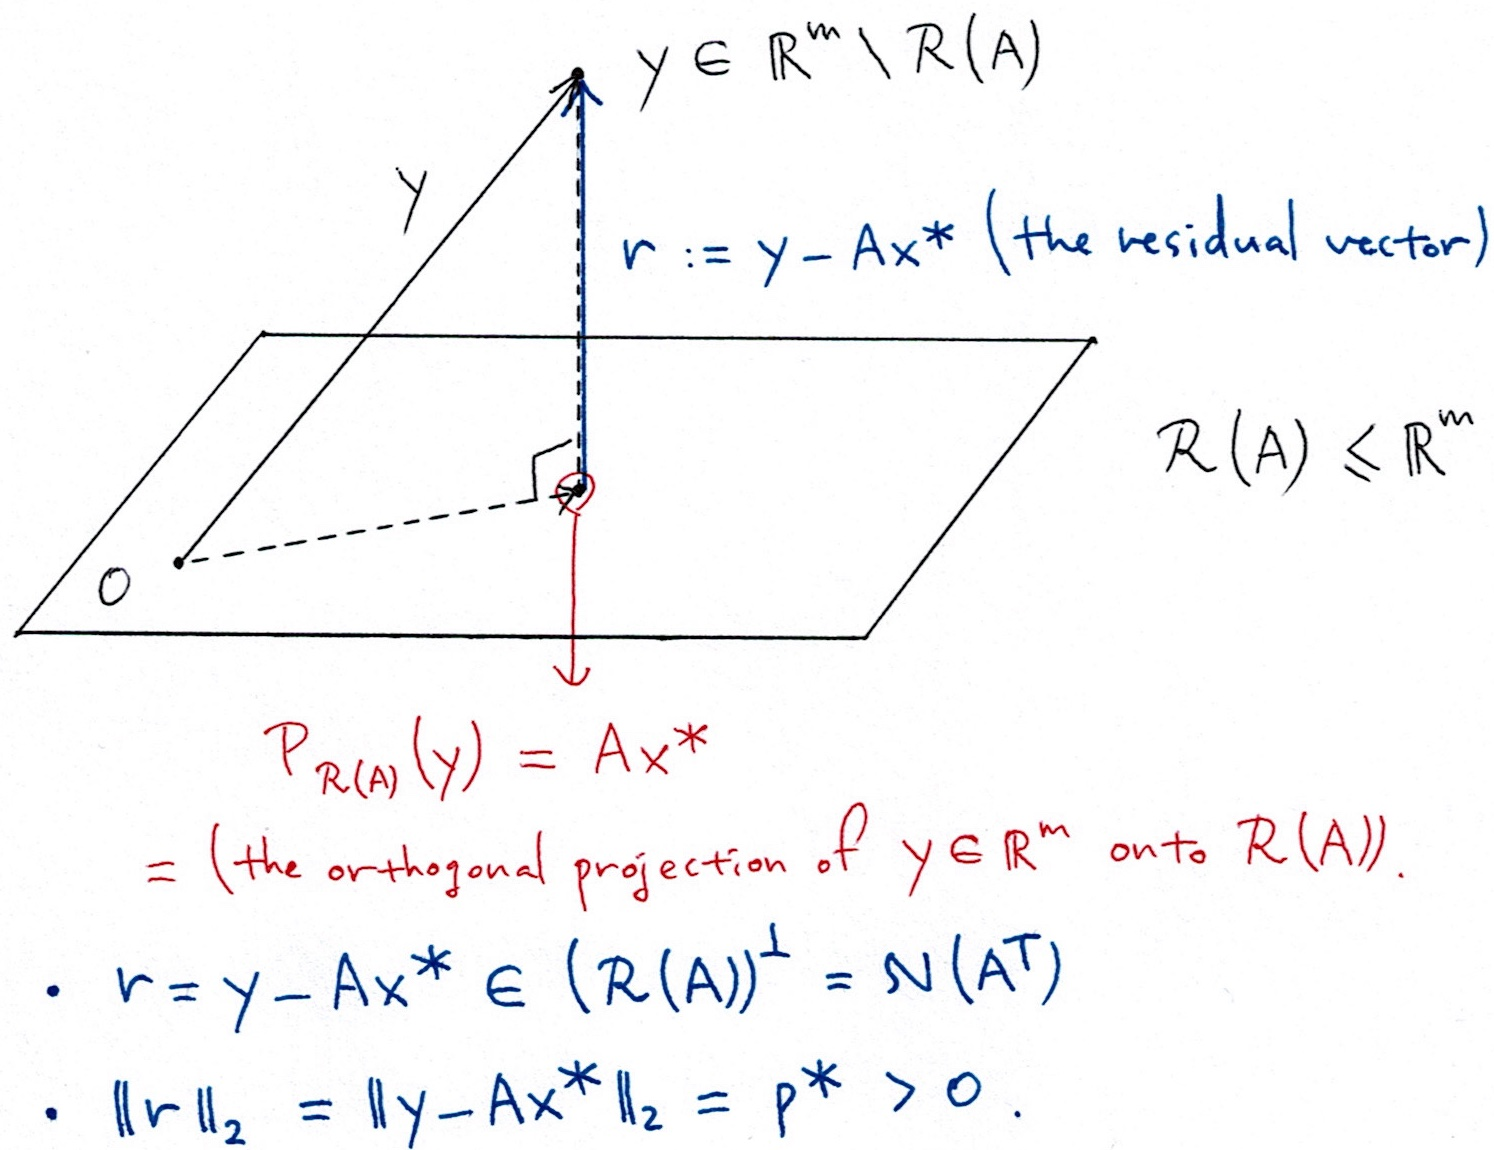
\includegraphics[width=0.6\textwidth]{HW4/figure_problem2.jpg}
    \caption{Geometric interpretation of the least-squares problem}
    \label{fig:problem_2}
\end{figure}

\indent As Figure \ref{fig:problem_2} shows, the property (\romannumeral 2) $\mathbf{A}^{\top} \mathbf{r} = \mathbf{0}$ asserts that the residual vector $\mathbf{r} = \mathbf{y} - \mathbf{A} \mathbf{x}^*$ is orthogonal to the range $\mathcal{R}(\mathbf{A})$ of $\mathbf{A} \in \mathbb{R}^{m \times n}$ since $\left( \mathcal{R}(\mathbf{A}) \right)^{\perp} = \mathcal{N} \left( \mathbf{A}^{\top} \right)$. Also, the property (\romannumeral 1) $\mathbf{r}^{\top} \mathbf{y} > 0$ can be interpreted as follows: let $\theta \in \left[ 0, \pi \right]$ denote the angle between two vectors $\mathbf{y} \in \mathbb{R}^m \setminus \mathcal{R} (\mathbf{A})$ and $\mathbf{r} \in \mathbb{R}^m \setminus \left\{ \mathbf{0} \right\}$, \emph{i.e.},
\begin{equation*}
    \cos \theta = \frac{\mathbf{r}^{\top} \mathbf{y}}{\left\| \mathbf{r} \right\|_2 \cdot \left\| \mathbf{y} \right\|_2}.
\end{equation*}
The property (\romannumeral 1) $\mathbf{r}^{\top} \mathbf{y} > 0$ implies $\cos \theta > 0$, which is equivalent to $\theta \in \left( 0, \frac{\pi}{2} \right)$. In other words, the property (\romannumeral 1) asserts that for two vectors $\mathbf{y}$ and $\mathbf{r}$ in $\mathbb{R}^m$, each vector has a component in the direction of the other.

}
\end{problem}

\begin{problem} [\emph{Exercise 6.4} in \cite{calafiore2014optimization}: Regularization for noisy data]
\label{problem3}
\normalfont{\ \\
\indent Let $\hat{\mathbf{a}}_1, \hat{\mathbf{a}}_2, \cdots, \hat{\mathbf{a}}_m \in \mathbb{R}^n$ and $\mathbf{u}_1, \mathbf{u}_2, \cdots, \mathbf{u}_m$ be $n$-dimensional random vectors such that
\begin{equation}
    \label{eqn3.1}
    \mathbb{E} \left[ \mathbf{u}_i \right] = \mathbf{0} \in \mathbb{R}^n \quad \textnormal{and} \quad
    \textsf{Cov} \left[ \mathbf{u}_i \right] = \mathbb{E} \left[ \mathbf{u}_i \mathbf{u}_{i}^{\top} \right] = \sigma^2 \mathbf{I}_n
\end{equation}
for every $i \in [m]$. Let $\mathbf{a}_i = \hat{\mathbf{a}}_i + \mathbf{u}_i$ for $i \in [m]$, $\mathbf{u} := \left( \mathbf{u}_1, \mathbf{u}_2, \cdots, \mathbf{u}_m \right)$, and
\begin{equation*}
    \hat{\mathbf{A}} :=
    \begin{bmatrix}
        \hat{\mathbf{a}}_{1}^{\top} \\
        \hat{\mathbf{a}}_{2}^{\top} \\
        \vdots \\
        \hat{\mathbf{a}}_{m}^{\top} \\
    \end{bmatrix}
    \in \mathbb{R}^{m \times n}; \quad
    \mathbf{U} :=
    \begin{bmatrix}
        \mathbf{u}_{1}^{\top} \\
        \mathbf{u}_{2}^{\top} \\
        \vdots \\
        \mathbf{u}_{m}^{\top} \\
    \end{bmatrix}; \quad
    \mathbf{A} = \mathbf{A} (\mathbf{u}) :=
    \begin{bmatrix}
        \mathbf{a}_{1}^{\top} \\
        \mathbf{a}_{2}^{\top} \\
        \vdots \\
        \mathbf{a}_{m}^{\top} \\
    \end{bmatrix}
    = \hat{\mathbf{A}} + \mathbf{U}.
\end{equation*}
Then both $\mathbf{U}$ and $\mathbf{A}$ are $m \times n$ real random matrices. One can observe that the objective function of the given original optimization problem satisfies
\begin{equation*}
    \begin{split}
        \mathbb{E}_{\mathbf{u}} \left[ \left\| \mathbf{A} (\mathbf{u}) \mathbf{x} - \mathbf{y} \right\|_{2}^2 \right]
        &= \mathbb{E}_{\mathbf{u}} \left[ \left\{ \left( \hat{\mathbf{A}} + \mathbf{U} \right) \mathbf{x} - \mathbf{y} \right\}^{\top} \left\{ \left( \hat{\mathbf{A}} + \mathbf{U} \right) \mathbf{x} - \mathbf{y} \right\} \right] \\
        &= \mathbb{E}_{\mathbf{u}} \left[ \mathbf{x}^{\top} \left( \hat{\mathbf{A}} + \mathbf{U} \right)^{\top} \left( \hat{\mathbf{A}} + \mathbf{U} \right) \mathbf{x} - 2 \mathbf{y}^{\top} \left( \hat{\mathbf{A}} + \mathbf{U} \right) \mathbf{x} + \mathbf{y}^{\top} \mathbf{y} \right] \\
        &= \mathbf{x}^{\top} \mathbb{E}_{\mathbf{u}} \left[ \left( \hat{\mathbf{A}} + \mathbf{U} \right)^{\top} \left( \hat{\mathbf{A}} + \mathbf{U} \right) \right] \mathbf{x} - 2 \mathbf{y}^{\top} \mathbb{E}_{\mathbf{u}} \left[ \hat{\mathbf{A}} + \mathbf{U} \right] \mathbf{x} + \mathbf{y}^{\top} \mathbf{y} \\
        &= \mathbf{x}^{\top} \left( \hat{\mathbf{A}}^{\top} \hat{\mathbf{A}} + \mathbb{E}_{\mathbf{u}} \left[ \mathbf{U} \right]^{\top} \hat{\mathbf{A}} + \hat{\mathbf{A}}^{\top} \mathbb{E}_{\mathbf{u}} \left[ \mathbf{U} \right] + \mathbb{E}_{\mathbf{u}} \left[ \mathbf{U}^{\top} \mathbf{U} \right] \right) \mathbf{x} - 2 \mathbf{y}^{\top} \left( \hat{\mathbf{A}} + \mathbb{E}_{\mathbf{u}} \left[ \mathbf{U} \right] \right) \mathbf{x} + \mathbf{y}^{\top} \mathbf{y} \\
        &\stackrel{\textnormal{(a)}}{=} \mathbf{x}^{\top} \left( \hat{\mathbf{A}}^{\top} \hat{\mathbf{A}} + \mathbb{E}_{\mathbf{u}} \left[ \mathbf{U}^{\top} \mathbf{U} \right] \right) \mathbf{x} - 2 \mathbf{y}^{\top} \hat{\mathbf{A}} \mathbf{x} + \mathbf{y}^{\top} \mathbf{y} \\
        &\stackrel{\textnormal{(b)}}{=} \left( \mathbf{x}^{\top}  \hat{\mathbf{A}}^{\top} \hat{\mathbf{A}} \mathbf{x} - 2 \mathbf{y}^{\top} \hat{\mathbf{A}} \mathbf{x} + \mathbf{y}^{\top} \mathbf{y} \right) + m \sigma^2 \cdot \mathbf{x}^{\top} \mathbf{I}_n \mathbf{x} \\
        &= \left\| \hat{\mathbf{A}} \mathbf{x} - \mathbf{y} \right\|_{2}^2 + m \sigma^2 \left\| \mathbf{x} \right\|_{2}^2,
    \end{split}
\end{equation*}
where the step (a) holds due to the fact $\mathbb{E}_{\mathbf{u}} \left[ \mathbf{U} \right] = \mathbf{O}_{m \times n}$, where $\mathbf{O}_{m \times n}$ denotes the $m \times n$ zero matrix, and the step (b) follows from the following observation:
\begin{equation*}
    \mathbb{E}_{\mathbf{u}} \left[ \mathbf{U}^{\top} \mathbf{U} \right] =
    \mathbb{E}_{\mathbf{u}} \left[ \sum_{i=1}^{m} \mathbf{u}_i \mathbf{u}_{i}^{\top} \right]
    = \sum_{i=1}^{m} \mathbb{E}_{\mathbf{u}} \left[ \mathbf{u}_i \mathbf{u}_{i}^{\top} \right]
    \stackrel{\textnormal{(c)}}{=} \sum_{i=1}^{m} \sigma^2 \mathbf{I}_n
    = m \sigma^2 \mathbf{I}_n,
\end{equation*}
where the step (c) comes from the assumption \eqref{eqn3.1}. Hence, the original optimization problem
\begin{equation*}
    \min_{\mathbf{x} \in \mathbb{R}^n} \ \mathbb{E}_{\mathbf{u}} \left[ \left\| \mathbf{A} (\mathbf{u}) \mathbf{x} - \mathbf{y} \right\|_{2}^2 \right]
\end{equation*}
can be written as the following regularized least-squares problem with the regularization parameter $\lambda = m \sigma^2$:
\begin{equation*}
    \min_{\mathbf{x} \in \mathbb{R}^n} \ \left( \left\| \hat{\mathbf{A}} \mathbf{x} - \mathbf{y} \right\|_{2}^2 + m \sigma^2 \left\| \mathbf{x} \right\|_{2}^2 \right).
\end{equation*}
}
\end{problem}

\begin{problem} [\emph{Exercise 8.1} in \cite{calafiore2014optimization}: Quadratic inequalities]
\label{problem4}
\normalfont{\ \\
\indent To begin with, let $\Omega \subseteq \mathbb{R}^2$ be a subset of $\mathbb{R}^2$ defined by
\begin{equation}
    \label{eqn4.1}
    \begin{split}
        \Omega &:= \left\{ \left( x_1, x_2 \right) \in \mathbb{R}^2 : x_2 \left( x_1 - x_2 + 1 \right) \geq 0 \right\} \\
        &= \left\{ \left( x_1, x_2 \right) \in \mathbb{R}^2 : x_1 \geq x_2 - 1 \textnormal{ and } x_2 \geq 0 \right\}
        \cup \left\{ \left( x_1, x_2 \right) \in \mathbb{R}^2 : x_1 \leq x_2 - 1 \textnormal{ and } x_2 \leq 0 \right\}.
    \end{split}
\end{equation}
\medskip

\indent (1) We first plot the region $\Omega$ explicitly:
\begin{figure}[h]
    \centering
    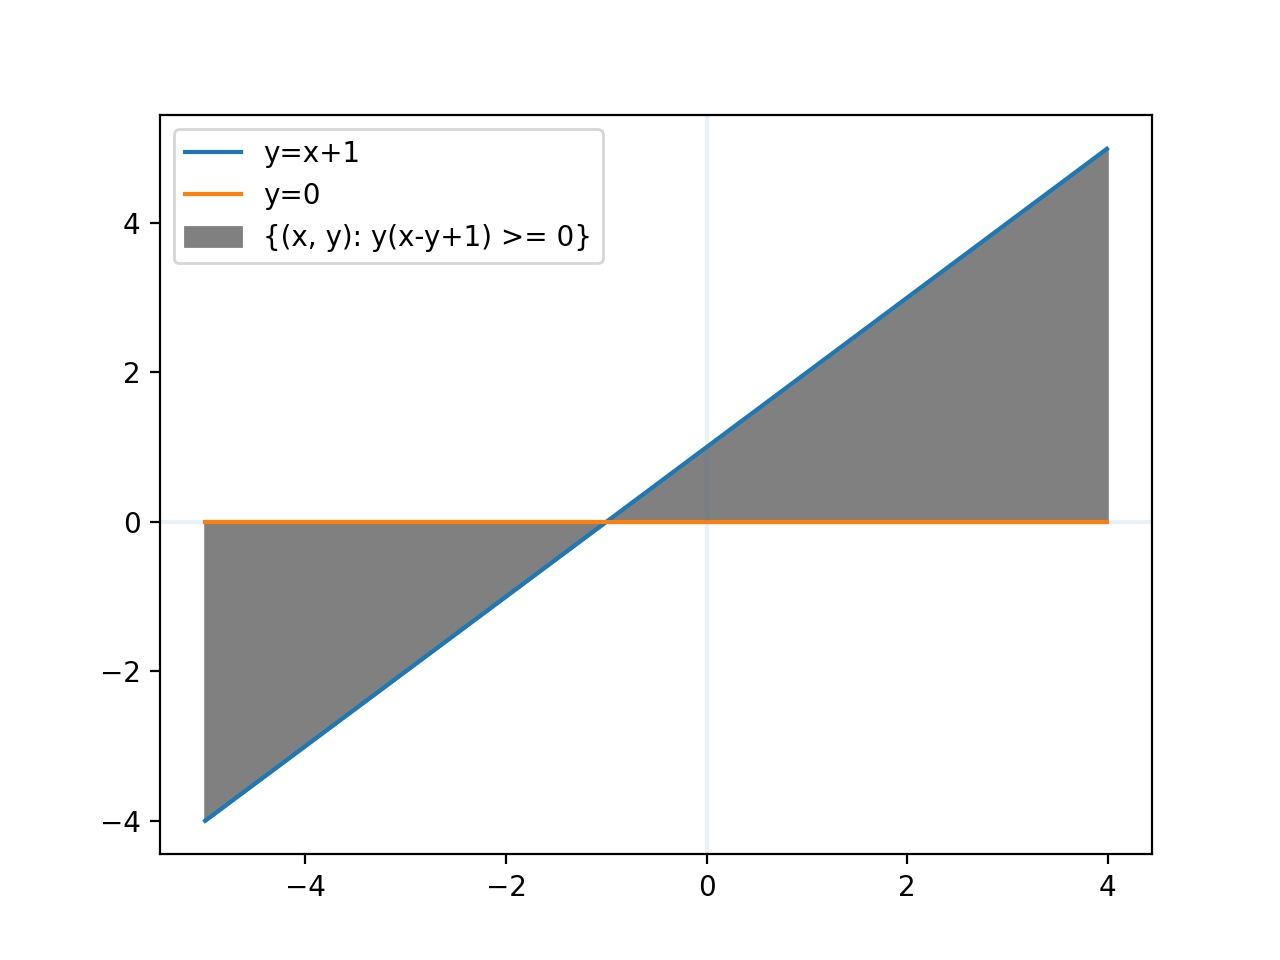
\includegraphics[width=0.6\textwidth]{HW4/figure_problem4.jpg}
    \caption{Visualization of the region $\Omega \subseteq \mathbb{R}^2$}
    \label{fig:problem_4}
\end{figure}

\noindent In the above figure, the region \eqref{eqn4.1} is filled with grey color. Now, we claim that $\Omega$ is not convex in $\mathbb{R}^2$. To this end, assume on the contrary that $\Omega$ is a convex subset of $\mathbb{R}^2$. Since $(0, 0) \in \Omega$ and $(-2, -1) \in \Omega$, the closed line segment $\left\{ (1-t) (0, 0) + t (-2, -1) : t \in [0, 1] \right\}$ connecting these two points should be contained in $\Omega$. However, the midpoint of those two points $\frac{1}{2} \left\{ (0, 0) + (-2, -1) \right\} = \left( -1, - \frac{1}{2} \right)$ does not belong to $\Omega$, \emph{i.e.},
\begin{equation*}
    \left( -1, - \frac{1}{2} \right) \in \mathbb{R}^2 \setminus \Omega,
\end{equation*}
and this yields a contradiction. Hence, the subset $\Omega$ of $\mathbb{R}^2$ is not convex!
\medskip

\indent (2) We begin with the following expression of the region $\Omega \subseteq \mathbb{R}^2$:
\begin{equation*}
    \Omega = \left\{ \left( x_1, x_2 \right) \in \mathbb{R}^2 : x_2 \left( x_2 - x_1 - 1 \right) \leq 0 \right\}.
\end{equation*}
One can observe that
\begin{equation}
    \label{eqn4.2}
    \begin{split}
        q (\mathbf{x})
        &:= x_2 \left( x_2 - x_1 - 1 \right) \\
        &= - x_1 x_2 + x_{2}^2 - x_2 \\
        &= \begin{bmatrix} x_1 & x_2 \end{bmatrix}
        \begin{bmatrix}
            0 & - \frac{1}{2} \\ - \frac{1}{2} & 1
        \end{bmatrix}
        \begin{bmatrix} x_1 \\ x_2 \end{bmatrix}
        + 2 \begin{bmatrix} 0 & - \frac{1}{2} \end{bmatrix}
        \begin{bmatrix} x_1 \\ x_2 \end{bmatrix} \\
        &= \mathbf{x}^{\top} \mathbf{A} \mathbf{x} + 2 \mathbf{b}^{\top} \mathbf{x} + c,
    \end{split}
\end{equation}
where $\mathbf{x} := \begin{bmatrix} x_1 \\ x_2 \end{bmatrix} \in \mathbb{R}^2$, $\mathbf{A} := \begin{bmatrix} 0 & - \frac{1}{2} \\ - \frac{1}{2} & 1 \end{bmatrix} \in \mathcal{S}^2$, $\mathbf{b} := \begin{bmatrix} 0 \\ - \frac{1}{2} \end{bmatrix} \in \mathbb{R}^2$, and $c := 0 \in \mathbb{R}$. Here, $\mathcal{S}^n$ denotes the set of all $n \times n$ real symmetric matrices. Hence, we have from \eqref{eqn4.2} that
\begin{equation*}
    \Omega = \left\{ \mathbf{x} \in \mathbb{R}^2 : q (\mathbf{x}) = \mathbf{x}^{\top} \mathbf{A} \mathbf{x} + 2 \mathbf{b}^{\top} \mathbf{x} + c \leq 0 \right\},
\end{equation*}
with the above choice of $\left( \mathbf{A}, \mathbf{b}, c \right) \in \mathcal{S}^2 \times \mathbb{R}^2 \times \mathbb{R}$, as desired.
\medskip

\indent (3) Given any subset $S$ of $\mathbb{R}^2$, let $\textsf{conv}(S)$ denote the convex hull of $S$ in $\mathbb{R}^2$:
\begin{equation*}
    \textsf{conv}(S) := \left\{ \sum_{k=1}^{n} \alpha_k \mathbf{x}_k : n \in \mathbb{N}, \mathbf{x}_1, \mathbf{x}_2, \cdots, \mathbf{x}_n \in S, \textnormal{ and } \alpha_k \geq 0,\ \forall k \in [n] \textnormal{ such that } \sum_{k=1}^{n} \alpha_k = 1 \right\}.
\end{equation*}
We claim that $\textsf{conv}(\Omega) = \mathbb{R}^2$. To this end, we will show that every point in $\mathbb{R}^2$ can be written as a convex combination of two points in $\Omega$. From the definition of convex hull, it's evident that this assertion establishes our desired conclusion $\textsf{conv}(\Omega) = \mathbb{R}^2$.
\medskip

\indent Choose and fix any point $\left( u_0, v_0 \right) \in \mathbb{R}^2$. If $\left( u_0, v_0 \right) \in \Omega$, then $\left( u_0, v_0 \right)$ is clearly a convex combination of two points $\left( u_0, v_0 \right) \in \Omega$ and $\left( u_0, v_0 \right) \in \Omega$. So we may assume that $\left( u_0, v_0 \right) \in \mathbb{R}^2 \setminus \Omega$, \emph{i.e.},
\begin{equation}
    \label{eqn4.3}
    v_0 \left( u_0 - v_0 + 1 \right) < 0.
\end{equation}
Now, let us consider the affine line $\left\{ \left( x_1, x_2 \right) \in \mathbb{R}^2 : x_2 - v_0 = \frac{1}{2} \left( x_1 - u_0 \right) \right\}$ in $\mathbb{R}^2$ which passes through the point $\left( u_0, v_0 \right) \in \mathbb{R}^2 \setminus \Omega$ and has slope $\frac{1}{2}$. Intuitively, this affine line should have intersections with affine lines $\left\{ \left( x_1, x_2 \right) \in \mathbb{R}^2 : x_2 = x_1 + 1 \right\}$ as well as $\left\{ \left( x_1, x_2 \right) \in \mathbb{R}^2 : x_2 = 0 \right\}$, which form the boundary of the region $\Omega$. To be precise, some straightforward calculations give
\begin{equation*}
    \begin{split}
        \left\{ \left( x_1, x_2 \right) \in \mathbb{R}^2 : x_2 - v_0 = \frac{1}{2} \left( x_1 - u_0 \right) \right\} \cap \left\{ \left( x_1, x_2 \right) \in \mathbb{R}^2 : x_2 = x_1 + 1 \right\} 
        &= \left\{ \left( 2v_0 - u_0 - 2, 2v_0 - u_0 - 1 \right) \right\}; \\
        \left\{ \left( x_1, x_2 \right) \in \mathbb{R}^2 : x_2 - v_0 = \frac{1}{2} \left( x_1 - u_0 \right) \right\} \cap \left\{ \left( x_1, x_2 \right) \in \mathbb{R}^2 : x_2 = 0 \right\} &=
        \left\{ \left( u_0 - 2v_0, 0 \right) \right\}.
    \end{split}
\end{equation*}
It's clear that $\left( 2v_0 - u_0 - 2, 2v_0 - u_0 - 1 \right) \in \Omega$ and $\left( u_0 - 2v_0, 0 \right) \in \Omega$. Intuitively, one can anticipate that $\left( u_0, v_0 \right)$ would lie in the closed line segment connecting these two points. In order to make this intuition rigorous, we observe that
\begin{equation}
    \label{eqn4.4}
    \left( u_0, v_0 \right) = \left\{ 1 - \theta^* \left( u_0, v_0 \right) \right\} \left( 2v_0 - u_0 - 2, 2v_0 - u_0 - 1 \right) + \theta^* \left( u_0, v_0 \right) \left( u_0 - 2v_0, 0 \right),
\end{equation}
where $\theta^* \left( u_0, v_0 \right) := \frac{u_0 - v_0 + 1}{u_0 - 2 v_0 + 1}$.

\begin{claim}
\label{claim1}
If $\left( u_0, v_0 \right) \in \mathbb{R}^2 \setminus \Omega$, then $\theta^* \left( u_0, v_0 \right) \in \left( 0, 1 \right)$.
\end{claim}

\begin{proof} [Proof of Claim \ref{claim1}]
The inequality \eqref{eqn4.3} will play a crucial role in the proof of Claim \ref{claim1}.
\begin{itemize}
    \item The case $v_0 > 0$: automatically, we have $u_0 - v_0 + 1 < 0$. This leads to $0 < v_0 - u_0 - 1 < 2 v_0 - u_0 - 1$, thereby
    \begin{equation*}
        0 < \theta^* \left( u_0, v_0 \right) = \frac{v_0 - u_0 - 1}{2 v_0 - u_0 - 1} < 1.
    \end{equation*}
    \item The case $v_0 < 0$: automatically, we have $u_0 - v_0 + 1 > 0$. This yields $0 < u_0 - v_0 + 1 < u_0 - 2v_0 + 1$, so
    \begin{equation*}
        0 < \theta^* \left( u_0, v_0 \right) = \frac{u_0 - v_0 + 1}{u_0 - 2 v_0 + 1} < 1.
    \end{equation*}
\end{itemize}
This completes the proof of Claim \ref{claim1}.

\end{proof}

\indent By combining the equation \eqref{eqn4.4} together with Claim \ref{claim1}, it is possible to conclude that $\left( u_0, v_0 \right) \in \mathbb{R}^2 \setminus \Omega$ can be written as a convex combination of two points $\left( 2v_0 - u_0 - 2, 2v_0 - u_0 - 1 \right) \in \Omega$ and $\left( u_0 - 2v_0, 0 \right) \in \Omega$. Therefore, we have $\mathbb{R}^2 \subseteq \textsf{conv}(\Omega) \subseteq \mathbb{R}^2$, and this establishes
\begin{equation*}
    \mathbb{R}^2 = \textsf{conv}(\Omega),
\end{equation*}
as desired.
}
\end{problem}

\newpage

\bibliographystyle{plain}
\bibliography{main.bib}

\end{document}
